% =============================================================================
%  PROIECT DE DIPLOMA
%  "Comparare algoritmi de predictie cu invatare automata"
%  Autor: Razvan-Bucur HOADREA
%
%  COMPILARE (recomandat XeLaTeX, pentru Times New Roman si Consolas reale):
%     xelatex lucrare.tex
%     biber   lucrare
%     xelatex lucrare.tex
%     xelatex lucrare.tex
%
%  Necesita: TeX Live / MiKTeX cu pachetele fontspec, babel-romanian, biblatex,
%  biber, listings, tikz, booktabs, caption. Fonturile Times New Roman si
%  Consolas exista implicit pe Windows.
% =============================================================================
% !TeX program = xelatex
% !BIB program = biber
\documentclass[12pt,a4paper]{report}

% --- Fonturi (XeLaTeX) -------------------------------------------------------
% Foloseste Times New Roman / Consolas DACA sunt instalate (local, pe Windows);
% altfel cade automat pe clone livrate cu orice distributie TeX -> merge si pe
% Overleaf, fara scanare lenta de fonturi (cauza probabila a timeout-ului).
\usepackage{fontspec}
\IfFontExistsTF{Times New Roman}{\setmainfont{Times New Roman}}{%
  \IfFontExistsTF{TeXGyreTermes}{\setmainfont{TeXGyreTermes}}{%
    \IfFontExistsTF{Tinos}{\setmainfont{Tinos}}{\setmainfont{Latin Modern Roman}}}}
\IfFontExistsTF{Consolas}{\setmonofont{Consolas}}{%
  \IfFontExistsTF{Inconsolata}{\setmonofont{Inconsolata}}{%
    \IfFontExistsTF{DejaVu Sans Mono}{\setmonofont{DejaVu Sans Mono}}{\setmonofont{Latin Modern Mono}}}}

% --- Limba romana ------------------------------------------------------------
\usepackage[romanian]{babel}

% --- Geometrie pagina: margini 2 cm ------------------------------------------
\usepackage[a4paper,margin=2cm]{geometry}

% --- Spatiere: 1.5 randuri, paragrafe cu "space before" 12pt -----------------
\usepackage{setspace}
\onehalfspacing
\setlength{\parindent}{0pt}
\setlength{\parskip}{12pt plus 2pt minus 1pt}

% --- Matematica --------------------------------------------------------------
\usepackage{amsmath,amssymb}

% --- Figuri ------------------------------------------------------------------
\usepackage{graphicx}
\graphicspath{{../outputs/plots/}{../outputs/}{figuri/}}

% --- Tabele ------------------------------------------------------------------
\usepackage{booktabs}
\usepackage{array}
\usepackage{enumitem}

% --- Captioane ---------------------------------------------------------------
% Figuri: "Figura X.Y Titlu", centrate sub figura.
% Tabele: "Tabelul X.Y Titlu", aliniate la stanga deasupra tabelului.
\usepackage{caption}
\captionsetup[figure]{labelsep=space, font=small, justification=centering, singlelinecheck=true, labelfont=bf, position=bottom}
\captionsetup[table]{labelsep=space, font=small, justification=raggedright, singlelinecheck=false, labelfont=bf, position=top}
\addto\captionsromanian{%
  \renewcommand{\figurename}{Figura}%
  \renewcommand{\tablename}{Tabelul}%
}

% --- Culori pentru listarile de cod ------------------------------------------
\usepackage{xcolor}
\definecolor{codecomment}{rgb}{0.00,0.50,0.00}
\definecolor{codekeyword}{rgb}{0.13,0.29,0.65}
\definecolor{codestring}{rgb}{0.64,0.08,0.08}
\definecolor{codenumber}{rgb}{0.50,0.50,0.50}
\definecolor{codeframe}{rgb}{0.80,0.80,0.80}

% --- Listari de cod: Consolas 10pt, fundal alb, 1 rand, syntax highlight -----
\usepackage{etoolbox}
\usepackage{listings}
% Codul se afiseaza la 1 rand (interlinie simpla), restul lucrarii la 1.5.
\BeforeBeginEnvironment{lstlisting}{\begin{singlespace}}
\AfterEndEnvironment{lstlisting}{\end{singlespace}}
\lstdefinestyle{python}{
  language=Python,
  backgroundcolor=\color{white},
  basicstyle=\ttfamily\fontsize{10pt}{12pt}\selectfont,
  commentstyle=\color{codecomment}\itshape,
  keywordstyle=\color{codekeyword}\bfseries,
  stringstyle=\color{codestring},
  numbers=left,
  numberstyle=\tiny\color{codenumber},
  numbersep=8pt,
  frame=single,
  rulecolor=\color{codeframe},
  breaklines=true,
  breakatwhitespace=true,
  keepspaces=true,
  showstringspaces=false,
  tabsize=4,
  captionpos=b,
  xleftmargin=14pt,
  aboveskip=10pt,
  belowskip=10pt,
  extendedchars=true,
}
\lstset{style=python}
\renewcommand{\lstlistingname}{Listarea}  % "Listarea X.Y"

% --- Diagrame (schema de arhitectura) ----------------------------------------
\usepackage{tikz}
\usetikzlibrary{shapes.geometric, arrows.meta, positioning, fit, backgrounds}

% --- Referinte / hyperlinkuri ------------------------------------------------
\usepackage[hidelinks]{hyperref}

% --- Bibliografie IEEE prin biblatex/biber -----------------------------------
\usepackage{csquotes}
\usepackage[backend=biber, style=ieee, sorting=none]{biblatex}
\addbibresource{referinte.bib}

% --- Numerotare: ecuatii pe capitol (X.Y); figurile/tabelele o fac implicit ---
% \counterwithin face parte din nucleul LaTeX (>= 2018), nu necesita pachet.
\counterwithin{equation}{chapter}
\setcounter{secnumdepth}{3}
\setcounter{tocdepth}{2}

% =============================================================================
\begin{document}

% -------------------------- PAGINI DE INCEPUT --------------------------------
% Primele trei pagini au fost inlocuite conform modelului furnizat.
\newgeometry{top=2cm,bottom=2cm,left=2cm,right=2cm}
\pagestyle{empty}
\begingroup
\singlespacing
\setlength{\parindent}{0pt}
\setlength{\parskip}{0pt}

% ================= COPERTA =================
\begin{titlepage}
\thispagestyle{empty}

\begin{center}

\vspace*{1.5cm}

\vspace{0.6cm}

UNIVERSITATEA ``LUCIAN BLAGA'' DIN SIBIU\\
FACULTATEA DE INGINERIE\\
DEPARTAMENTUL DE CALCULATOARE ȘI INGINERIE ELECTRICĂ

\vspace{6.5cm}

{\LARGE \textbf{PROIECT DE DIPLOMĂ}}

\end{center}

\vspace{2.4cm}

\noindent
\begin{minipage}{0.75\textwidth}
Conducător științific: Șef lucr. Alexandru DOROBANȚIU\\
Îndrumător: Șef lucr. Alexandru DOROBANȚIU
\end{minipage}

\vspace{2.5cm}

\hspace*{8.2cm}
\begin{minipage}{0.45\textwidth}
Absolvent:\\
Răzvan-Bucur HOADREA\\
Specializarea CALCULATOARE
\end{minipage}

\vfill

\begin{center}
-\quad Sibiu, 2026 -
\end{center}

\vspace{1.2cm}

\end{titlepage}

% ================= PAGINA DUPĂ COPERTĂ =================
\begin{titlepage}
\thispagestyle{empty}

\begin{center}

\vspace*{1.2cm}

\vspace{0.6cm}

UNIVERSITATEA ``LUCIAN BLAGA'' DIN SIBIU\\
FACULTATEA DE INGINERIE\\
DEPARTAMENTUL DE CALCULATOARE ȘI INGINERIE ELECTRICĂ

\vspace{6.8cm}

{\LARGE \textbf{TITLUL TEMEI}}

\vspace{0.6cm}

\textbf{Comparare algoritmi de predicție cu învățare automată}

\end{center}

\vspace{4.3cm}

\noindent
\begin{minipage}{0.75\textwidth}
Conducător științific: Șef lucr. Alexandru DOROBANȚIU\\
Îndrumător: Șef lucr. Alexandru DOROBANȚIU
\end{minipage}

\vspace{2.6cm}

\hspace*{8.2cm}
\begin{minipage}{0.45\textwidth}
Absolvent:\\
Răzvan-Bucur HOADREA\\
Specializarea CALCULATOARE
\end{minipage}

\vfill

\end{titlepage}

% ================= PLAN TEMATIC =================
\begin{titlepage}
\thispagestyle{empty}

\fontsize{11}{13}\selectfont

\vspace*{1.2cm}

\noindent
\begin{minipage}[t]{0.58\textwidth}
\textbf{UNIVERSITATEA ``LUCIAN BLAGA'' DIN SIBIU}\\
\textbf{FACULTATEA DE INGINERIE}\\
\textbf{DEPARTAMENTUL DE CALCULATOARE}\\
\textbf{ȘI INGINERIE ELECTRICĂ}
\end{minipage}
\hfill
\begin{minipage}[t]{0.35\textwidth}
\centering
\textbf{APROBAT (data)}

\vspace{0.8cm}

\textbf{DIRECTOR DEPARTAMENT}

\vspace{0.5cm}

\rule{4cm}{0.4pt}
\end{minipage}

\vspace{1.8cm}

\begin{center}
\textbf{PLAN TEMATIC}\\
\textbf{pentru proiectul de diplomă}
\end{center}

\vspace{1.2cm}

\noindent
Proiectul de diplomă dat studentului: Răzvan-Bucur HOADREA

\vspace{0.6cm}

\noindent
\textbf{1. Tema proiectului:} Comparare algoritmi de predicție cu învățare automată

\vspace{0.5cm}

\noindent
\textbf{2. Termenul de predare a proiectului:} IUNIE 2026

\vspace{0.5cm}

\noindent
\textbf{3. Elemente inițiale pentru proiect:} Învățare automată, Benchmark competiție sportivă

\vspace{0.5cm}

\noindent
\textbf{4. Nota explicativă (enumerarea problemelor care vor fi rezolvate):}

\begin{itemize}[topsep=0pt,itemsep=0pt,leftmargin=1.2cm]
    \item Implementarea unui model de învățare automată
    \item Aplicare de predicții pe baza seturilor de date
    \item Efectuarea unui studiu comparativ între mai mulți algoritmi de învățare automată
\end{itemize}

\vspace{0.3cm}

\noindent
\textbf{5. Enumerarea materialului grafic (cu indicarea precisă a desenelor obligatorii):}

\begin{itemize}[topsep=0pt,itemsep=0pt,leftmargin=1.2cm]
    \item Schema arhitecturii algoritmilor de învățare automată
    \item Graficul comparativ al performanței algoritmilor
\end{itemize}

\vspace{0.3cm}

\noindent
\textbf{6. Consultații pentru proiect (săptămânal):} MIERCURI 14:00--15:00

\vspace{0.5cm}

\noindent
\textbf{7. Data eliberării temei:} OCTOMBRIE 2025.

\vspace{0.8cm}

\noindent
\begin{minipage}[t]{0.46\textwidth}
\textbf{Tema a fost primită pentru îndeplinire:}\\
\textbf{Data 31.10.2025}

\vspace{0.8cm}

\textbf{Semnătură student}

\vspace{0.9cm}

\rule{4cm}{0.4pt}

\vspace{1cm}

\textbf{(semnătura)}
\end{minipage}
\hfill
\begin{minipage}[t]{0.46\textwidth}
\centering
\textbf{CONDUCĂTOR,}\\
{\scriptsize \textbf{(grad didactic, prenume, nume)}}

\vspace{0.8cm}

\textbf{Șef lucr. Alexandru DOROBANȚIU}

\vspace{0.9cm}

\rule{4.5cm}{0.4pt}
\end{minipage}

\vfill

\end{titlepage}

\endgroup
\restoregeometry


% Numerotarea paginilor incepe cu cuprinsul.
\setcounter{page}{1}
\pagenumbering{arabic}
\pagestyle{plain}

% ------------------------------- CUPRINS -------------------------------------
\tableofcontents

% =============================================================================
\chapter{Introducere}
\label{cap:introducere}

\section{Prezentarea temei}

Predicția rezultatelor sportive este un domeniu de aplicație clasic pentru învățarea
automată, deoarece combină date structurate, abundente și actualizate periodic cu o
problemă de decizie clar definită. Formula 1 oferă un cadru deosebit de potrivit: fiecare
sezon generează zeci de curse, fiecare cursă produce rezultate pentru aproximativ douăzeci
de piloți, iar regulile competiției sunt stabile pe perioade de mai mulți ani. Spre
deosebire de sporturile de echipă, în care rezultatul depinde de interacțiuni complexe între
mulți jucători, în Formula 1 performanța individuală a pilotului și a echipei poate fi
urmărită numeric de la o cursă la alta.

Lucrarea de față abordează problema predicției \emph{podiumului} unei curse de Formula 1,
adică a identificării celor trei piloți care vor termina pe primele trei locuri (P1, P2 și
P3). Problema este formulată ca o sarcină de clasificare binară: pentru fiecare pereche
(cursă, pilot) se estimează probabilitatea ca pilotul respectiv să termine pe podium, după
care, pentru fiecare cursă, piloții sunt ordonați descrescător după această probabilitate,
iar primii trei formează podiumul prezis. Pe lângă predicția per cursă, probabilitățile sunt
agregate într-un clasament de campionat estimat la finalul sezonului.

Elementul central al lucrării nu este atât aplicația în sine, cât \textbf{studiul comparativ}
al trei algoritmi de învățare automată implementați integral, fără utilizarea unor
biblioteci de învățare automată gata făcute: regresia logistică, arborele de decizie și
pădurea aleatoare (\emph{Random Forest}). Implementarea de la zero, peste biblioteca de
calcul numeric NumPy~\cite{harris2020numpy}, urmărește înțelegerea în profunzime a
mecanismelor fiecărui algoritm și controlul complet asupra procesului de antrenare și
evaluare.

\section{Motivație}

Alegerea temei este motivată de trei aspecte. În primul rând, implementarea de la zero a
algoritmilor expune detaliile pe care bibliotecile consacrate, precum
scikit-learn~\cite{pedregosa2011scikit}, le ascund: coborârea pe gradient, criteriul de
divizare bazat pe entropie sau mecanismul de \emph{bagging}. În al doilea rând, datele din
Formula 1 ridică o provocare metodologică reală --- \emph{scurgerea de informație} (eng.
\emph{data leakage}) ---, deoarece orice caracteristică folosită pentru a prezice o cursă
trebuie calculată exclusiv din rezultate anterioare acelei curse. În al treilea rând,
distribuția claselor este puternic dezechilibrată (doar aproximativ 15\% dintre piloți
termină pe podium), ceea ce face ca metrica de acuratețe globală să fie
înșelătoare~\cite{he2009learning, saito2015precision} și impune folosirea unor metrici
adecvate.

\section{Scop și obiective}

Scopul lucrării este realizarea unui studiu comparativ riguros între trei algoritmi de
învățare automată aplicați aceleiași probleme de predicție, în condiții identice de
antrenare și evaluare. Obiectivele concrete, în acord cu planul tematic al proiectului,
sunt următoarele:

\begin{enumerate}
  \item \textbf{Implementarea de la zero} a trei modele de învățare automată (regresie
    logistică, arbore de decizie și pădure aleatoare), folosind doar NumPy pentru algebra
    vectorizată.
  \item \textbf{Aplicarea predicțiilor} pe un set de date real, alcătuit din rezultatele
    curselor de Formula 1 din sezoanele 2018--2025, cu o etapă de inginerie a
    caracteristicilor strict cauzală, fără scurgere de informație.
  \item \textbf{Efectuarea unui studiu comparativ} între cei trei algoritmi, atât din punctul
    de vedere al calității predicțiilor (acuratețe, F1, rată de nimerire a podiumului, arie
    sub curbele ROC și Precision-Recall), cât și al costului de calcul (timpul de antrenare).
  \item \textbf{Analiza hiperparametrilor} fiecărui model, prin curbe de validare și căutare
    pe grilă, pentru a justifica valorile alese.
\end{enumerate}

\section{Structura lucrării}

Lucrarea este organizată în cinci capitole. Capitolul~\ref{cap:teorie} prezintă fundamentele
teoretice ale învățării automate și ale celor trei algoritmi studiați, împreună cu metodele
de validare și metricile de evaluare. Capitolul~\ref{cap:rezolvare} descrie soluția
dezvoltată: arhitectura sistemului, sursa de date, ingineria caracteristicilor cauzale,
implementarea algoritmilor și a procedurii de validare. Capitolul~\ref{cap:rezultate}
prezintă și interpretează rezultatele experimentale. Capitolul~\ref{cap:concluzii} sintetizează
concluziile și propune direcții de dezvoltare ulterioară.

% =============================================================================
\chapter{Considerații teoretice}
\label{cap:teorie}

\section{Învățarea automată și clasificarea supervizată}

Învățarea automată studiază algoritmii care îmbunătățesc performanța la o sarcină pe baza
experienței, exprimată sub forma unor date~\cite{bishop2006pattern}. În cadrul \emph{învățării
supervizate}, algoritmul primește un set de exemple de antrenament
$\{(\mathbf{x}_i, y_i)\}_{i=1}^{n}$, unde $\mathbf{x}_i \in \mathbb{R}^d$ este un vector de
caracteristici, iar $y_i$ este eticheta asociată. Scopul este învățarea unei funcții
$f: \mathbb{R}^d \to \mathcal{Y}$ care generalizează bine pe date nevăzute.

Atunci când eticheta ia două valori, $\mathcal{Y} = \{0, 1\}$, problema se numește
\emph{clasificare binară}. În lucrarea de față, eticheta $y = 1$ semnifică faptul că pilotul
termină pe podium (locul $\leq 3$), iar $y = 0$ în caz contrar. Multe modele de clasificare
nu produc direct eticheta, ci o \emph{probabilitate} $\hat{p} = P(y = 1 \mid \mathbf{x})$, pe
care o transformă într-o etichetă printr-un prag de decizie (uzual $0{,}5$). Această
probabilitate este esențială în soluția propusă, fiindcă servește drept scor de ordonare a
piloților în cadrul fiecărei curse.

\section{Problema dezechilibrului de clase}
\label{sec:dezechilibru}

Un set de date este dezechilibrat atunci când clasele nu sunt reprezentate în proporții
apropiate. În cazul predicției podiumului, doar trei din aproximativ douăzeci de piloți
ajung pe podium în fiecare cursă, deci clasa pozitivă reprezintă circa 15\% din
exemple. În astfel de situații, un clasificator trivial care prezice mereu clasa majoritară
(``nu termină pe podium'') obține o acuratețe ridicată (aproximativ 85\%) fără a avea nicio
valoare practică~\cite{he2009learning}. De aceea, evaluarea trebuie completată cu metrici
care surprind performanța pe clasa minoritară, precum scorul F1 și aria sub curba
Precision-Recall~\cite{saito2015precision}. O tehnică suplimentară de atenuare a
dezechilibrului este ponderarea exemplelor pe clase în funcția de cost, aplicată în această
lucrare la regresia logistică.

\section{Regresia logistică}
\label{sec:logreg}

Regresia logistică modelează probabilitatea clasei pozitive printr-o transformare neliniară a
unei combinații liniare de caracteristici~\cite{hastie2009elements}. Fie $\mathbf{w}$ vectorul
de ponderi și $b$ termenul liber; modelul calculează scorul $z = \mathbf{w}^\top \mathbf{x} + b$
și îl transformă prin funcția \emph{sigmoid}:
\begin{equation}
  \sigma(z) = \frac{1}{1 + e^{-z}}, \qquad \hat{p} = \sigma(\mathbf{w}^\top \mathbf{x} + b).
  \label{eq:sigmoid}
\end{equation}

Antrenarea minimizează funcția de cost de tip \emph{entropie încrucișată} (eng.
\emph{cross-entropy}), la care se adaugă un termen de regularizare $L_2$ ce penalizează
ponderile mari și combate supraînvățarea:
\begin{equation}
  \mathcal{L}(\mathbf{w}, b) = -\frac{1}{N} \sum_{i=1}^{N} \Big[ y_i \log \hat{p}_i +
  (1 - y_i) \log (1 - \hat{p}_i) \Big] + \frac{\lambda}{2} \lVert \mathbf{w} \rVert_2^2 .
  \label{eq:bce}
\end{equation}

Minimizarea se realizează prin \emph{coborâre pe gradient} (eng. \emph{gradient descent}):
ponderile sunt actualizate iterativ în sensul opus gradientului, cu un pas de învățare $\eta$.
Gradientul funcției de cost față de ponderi are forma compactă:
\begin{equation}
  \nabla_{\mathbf{w}} \mathcal{L} = \frac{1}{N} \mathbf{X}^\top (\hat{\mathbf{p}} - \mathbf{y})
  + \lambda \mathbf{w}.
  \label{eq:gradient}
\end{equation}

Pentru a contracara dezechilibrul de clase (Secțiunea~\ref{sec:dezechilibru}), fiecare exemplu
poate primi o pondere invers proporțională cu frecvența clasei sale, astfel încât erorile pe
clasa minoritară (podium) să contribuie semnificativ la funcția de cost.

\section{Arbori de decizie}
\label{sec:tree}

Un arbore de decizie partiționează recursiv spațiul caracteristicilor prin teste de forma
``caracteristica $j$ este $\leq$ pragul $t$?''~\cite{breiman1984cart}. Fiecare nod intern
aplică un astfel de test, iar fiecare frunză stochează o predicție --- în cazul de față,
fracția de exemple pozitive din frunză, interpretată drept probabilitate de podium.

Criteriul de alegere a divizărilor folosit în această lucrare este \emph{câștigul de
informație} (eng. \emph{information gain}), bazat pe \emph{entropie}. Pentru un nod cu
proporția $p$ de exemple pozitive, entropia binară este:
\begin{equation}
  H(p) = -p \log_2 p - (1 - p) \log_2 (1 - p),
  \label{eq:entropie}
\end{equation}
cu convenția $0 \log_2 0 = 0$. Câștigul de informație al unei divizări care împarte un nod
părinte în doi copii (stânga și dreapta) este reducerea de entropie:
\begin{equation}
  IG = H(\text{părinte}) - \frac{n_{st}}{n} H(\text{stânga}) - \frac{n_{dr}}{n} H(\text{dreapta}).
  \label{eq:gain}
\end{equation}
Algoritmul alege, la fiecare nod, perechea (caracteristică, prag) care maximizează câștigul de
informație. Creșterea arborelui se oprește la atingerea unor criterii precum adâncimea maximă
(\texttt{max\_depth}), numărul minim de exemple necesare pentru divizare
(\texttt{min\_samples\_split}) sau numărul minim de exemple într-o frunză
(\texttt{min\_samples\_leaf}). Aceste criterii controlează compromisul dintre subînvățare și
supraînvățare.

\section{Pădurea aleatoare (Random Forest)}
\label{sec:forest}

Pădurea aleatoare este o metodă de tip ansamblu care combină predicțiile mai multor arbori de
decizie pentru a reduce varianța și a îmbunătăți generalizarea~\cite{breiman2001random}. Doi
factori de aleatoriu decorelează arborii:
\begin{itemize}
  \item \textbf{Bagging} (eng. \emph{bootstrap aggregating}): fiecare arbore este antrenat pe
    un eșantion bootstrap, obținut prin extragerea cu revenire a $n$ exemple din setul de
    antrenament.
  \item \textbf{Subset aleator de caracteristici}: la fiecare divizare se consideră doar un
    subset aleator de caracteristici (uzual $\sqrt{d}$), nu toate cele $d$ disponibile.
\end{itemize}
Predicția finală este media probabilităților produse de toți arborii. Un avantaj important al
metodei este estimarea \emph{out-of-bag} (OOB): pentru fiecare exemplu, predicția se calculează
folosind doar arborii care nu l-au inclus în eșantionul bootstrap, oferind o estimare a erorii
de generalizare fără un set de validare separat~\cite{breiman2001random}.

\section{Ingineria caracteristicilor și scurgerea de informație}
\label{sec:leakage}

Calitatea unui model de învățare automată depinde decisiv de caracteristicile de
intrare~\cite{james2013introduction}. În problemele cu o componentă temporală, precum
predicția unei curse viitoare, apare riscul de \emph{scurgere de informație}: utilizarea, la
antrenare, a unor informații care nu ar fi disponibile în momentul predicției reale. De
exemplu, folosirea numărului total de puncte acumulate de un pilot într-un sezon ar include
rezultatul cursei pe care încercăm să o prezicem.

Pentru a evita acest fenomen, toate caracteristicile trebuie să fie \emph{strict cauzale},
adică să folosească exclusiv informații anterioare cursei prezise. Strategia adoptată constă
în procesarea curselor în ordine cronologică și menținerea unei ``stări'' istorice, din care
se calculează caracteristicile înainte de a fi actualizată cu rezultatul cursei curente.

\section{Validarea și estimarea performanței}
\label{sec:validare}

Estimarea corectă a performanței necesită evaluarea modelului pe date care nu au fost folosite
la antrenare~\cite{kohavi1995study}. Validarea încrucișată clasică (\emph{k-fold}) presupune
însă că exemplele sunt independente și interschimbabile, ceea ce nu este valabil pentru date
temporale: nu putem antrena pe curse viitoare pentru a prezice curse trecute. De aceea, în
această lucrare se folosește o \emph{validare temporală pe ani} (eng. \emph{rolling
cross-year}): pentru fiecare sezon de test $S$, modelul este antrenat pe toate sezoanele
anterioare ($< S$) și evaluat pe sezonul $S$. Astfel se prezice mereu ``viitorul'' cu modele
antrenate doar pe ``trecut'', eliminând scurgerea de informație temporală.

\section{Metrici de evaluare}
\label{sec:metrici}

Pentru clasificarea binară, plecând de la numărul de adevărat pozitive (TP), fals pozitive
(FP), adevărat negative (TN) și fals negative (FN), se definesc:
\begin{align}
  \text{Acuratețe} &= \frac{TP + TN}{TP + TN + FP + FN}, &
  \text{Precizie} &= \frac{TP}{TP + FP}, \label{eq:acc}\\
  \text{Recall} &= \frac{TP}{TP + FN}, &
  F_1 &= \frac{2 \cdot \text{Precizie} \cdot \text{Recall}}{\text{Precizie} + \text{Recall}}.
  \label{eq:f1}
\end{align}
Scorul $F_1$ este media armonică dintre precizie și recall și este preferat acurateței în
prezența dezechilibrului de clase. Curba ROC reprezintă rata adevărat pozitivelor în funcție
de rata fals pozitivelor, la variația pragului de decizie; aria sub această curbă (AUC) este o
măsură agregată a capacității de discriminare~\cite{fawcett2006roc}. Curba Precision-Recall și
aria sub ea (\emph{average precision}, AP) sunt mai informative decât ROC atunci când clasa
pozitivă este rară~\cite{saito2015precision}. În fine, \emph{curba de calibrare} (eng.
\emph{reliability diagram}) compară probabilitatea medie prezisă cu frecvența reală observată,
indicând cât de bine pot fi interpretate probabilitățile ca atare~\cite{niculescu2005predicting}.

Pe lângă metricile de clasificare, soluția definește metrici specifice problemei, calculate la
nivel de cursă și apoi mediate: \emph{rata de nimerire a podiumului} (câți dintre cei trei
piloți preziși se regăsesc în podiumul real), acuratețea predicției câștigătorului și
suprapunerea cu primii trei din clasamentul de campionat.

\section{Lucrări conexe}

Aplicarea învățării automate la predicția rezultatelor sportive a fost studiată pe larg.
Bunker și Thabtah~\cite{bunker2019machine} propun un cadru general pentru predicția
rezultatelor sportive și subliniază importanța ingineriei caracteristicilor și a evaluării
temporale. Metodele de tip ansamblu, în special pădurile aleatoare, sunt frecvent raportate ca
fiind robuste și competitive pe date tabulare~\cite{breiman2001random, hastie2009elements}.
Lucrarea de față se diferențiază prin implementarea integrală a algoritmilor și prin accentul
pus pe analiza comparativă a hiperparametrilor și a costului de calcul.

% =============================================================================
\chapter{Rezolvarea temei de proiect}
\label{cap:rezolvare}

\section{Arhitectura sistemului}
\label{sec:arhitectura}

Sistemul este organizat ca o succesiune de etape (eng. \emph{pipeline}), de la datele brute
până la predicții și evaluare. Figura~\ref{fig:arhitectura} prezintă schema de arhitectură:
datele sunt încărcate din memoria cache locală, transformate într-un tabel de rezultate, apoi
îmbogățite cu caracteristici cauzale; pe acest set se antrenează cele trei modele, ale căror
probabilități sunt folosite atât pentru predicția podiumului per cursă, cât și pentru
agregarea în clasament și pentru modulul de evaluare și vizualizare.

\begin{figure}[htbp]
  \centering
  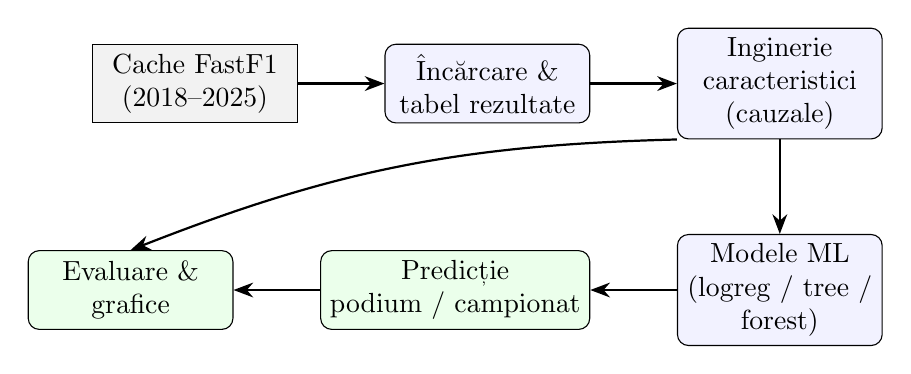
\begin{tikzpicture}[
      node distance=0.7cm and 1.1cm,
      box/.style={draw, rounded corners, align=center, minimum height=1cm,
                  minimum width=2.6cm, fill=blue!5},
      data/.style={draw, align=center, minimum height=1cm, minimum width=2.6cm, fill=gray!10},
      outputnode/.style={draw, rounded corners, align=center, minimum height=1cm,
                  minimum width=2.6cm, fill=green!8},
      arrow/.style={-{Stealth[length=2.5mm]}, thick}
    ]
    \node[data] (cache) {Cache FastF1\\(2018--2025)};
    \node[box, right=of cache] (loader) {Încărcare \&\\tabel rezultate};
    \node[box, right=of loader] (feat) {Inginerie\\caracteristici\\(cauzale)};
    \node[box, below=1.2cm of feat] (models) {Modele ML\\(logreg / tree /\\forest)};
    \node[outputnode, left=of models] (podium) {Predicție\\podium / campionat};
    \node[outputnode, left=of podium] (eval) {Evaluare \&\\grafice};

    \draw[arrow] (cache) -- (loader);
    \draw[arrow] (loader) -- (feat);
    \draw[arrow] (feat) -- (models);
    \draw[arrow] (models) -- (podium);
    \draw[arrow] (podium) -- (eval);
    \draw[arrow] (feat.south west) to[bend right=10] (eval.north);
  \end{tikzpicture}
  \caption{Arhitectura sistemului de predicție: de la datele brute la evaluare.}
  \label{fig:arhitectura}
\end{figure}

Implementarea este realizată în limbajul Python, organizată în pachetul \texttt{f1pred}.
Bibliotecile externe sunt folosite strict pentru sarcini auxiliare: NumPy~\cite{harris2020numpy}
pentru algebra vectorizată, pandas~\cite{mckinney2010pandas} pentru manipularea datelor
tabelare, matplotlib~\cite{hunter2007matplotlib} pentru grafice și
FastF1~\cite{fastf1} pentru încărcarea datelor. Niciuna nu este o bibliotecă de învățare
automată; toți algoritmii, metricile și procedura de antrenare sunt implementați manual.

\section{Sursa de date}

Datele provin din interfața de programare FastF1~\cite{fastf1}, care oferă acces la
rezultatele oficiale și la informațiile de cronometraj din Formula 1. Au fost folosite opt
sezoane (2018--2025), însumând aproximativ 3500 de rezultate (perechi cursă--pilot). Pentru
reproductibilitate și pentru a elimina dependența de conexiunea la internet, datele sunt
citite dintr-o memorie cache locală, în mod strict offline.

\section{Construirea setului de date}

Prima etapă transformă datele brute într-un tabel ``lung'', cu o linie pentru fiecare pereche
(sezon, rundă, pilot), conținând poziția pe grilă, poziția în calificări, poziția finală,
punctele, echipa și condițiile meteo. Tabelul este sortat cronologic --- pas esențial pentru
calculul corect al caracteristicilor rulante --- și salvat în format Parquet pentru reutilizare
rapidă.

\section{Ingineria caracteristicilor cauzale}
\label{sec:features}

Pe baza considerentelor din Secțiunea~\ref{sec:leakage}, au fost construite 30 de
caracteristici numerice, toate strict cauzale. Acestea se grupează în următoarele categorii,
rezumate în Tabelul~\ref{tab:features}: poziția pe grilă și în calificări (cunoscute înainte de
cursă), forma rulantă a pilotului (medii pe ultimele cinci curse), statistici cumulate la nivel
de sezon, forța echipei, istoricul pe circuitul respectiv și contextul cursei (experiență,
condiții meteo).

\begin{table}[htbp]
  \caption{Categoriile de caracteristici folosite de modele.}
  \label{tab:features}
  \begin{tabular}{l l c}
    \toprule
    \textbf{Categorie} & \textbf{Exemple de caracteristici} & \textbf{Nr.} \\
    \midrule
    Grilă / calificări     & poziție grilă, poziție calificări, pole                 & 5  \\
    Formă rulantă pilot    & medie sosire, medie puncte, rată podium, rată abandon   & 6  \\
    Sezon-to-date pilot    & puncte, poziție, podiumuri, victorii, curse             & 5  \\
    Forța echipei          & formă echipă, puncte echipă, poziție echipă             & 4  \\
    Istoric circuit        & medie sosire pilot / echipă, rată podium pe circuit     & 3  \\
    Context                & experiență, rundă, weekend cu sprint, vreme             & 7  \\
    \midrule
    \textbf{Total}         &                                                         & \textbf{30} \\
    \bottomrule
  \end{tabular}
\end{table}

Principiul cauzalității este implementat prin actualizarea stării istorice \emph{după}
calcularea caracteristicilor cursei curente. Listarea~\ref{lst:leakage} ilustrează această
ordine pentru caracteristica ``puncte acumulate în sezon'': valoarea atribuită cursei curente
reflectă doar cursele anterioare.

\begin{lstlisting}[caption={Actualizarea stării istorice dupa calcularea caracteristicilor (principiul anti-leakage).}, label={lst:leakage}]
# Pas 1: caracteristicile cursei R folosesc DOAR starea de pana acum.
row["season_points"] = state_points[driver]      # puncte inainte de cursa R

# Pas 2: abia DUPA ce s-au calculat caracteristicile,
#        starea este actualizata cu rezultatul cursei R.
state_points[driver] += points_in_race_R
\end{lstlisting}

\section{Implementarea regresiei logistice}

Regresia logistică (Secțiunea~\ref{sec:logreg}) a fost implementată prin coborâre pe gradient
în varianta \emph{batch}, cu regularizare $L_2$ și ponderare pe clase. Caracteristicile sunt
standardizate intern (medie zero, abatere standard unitară), parametrii standardizării fiind
învățați exclusiv pe datele de antrenament. Listarea~\ref{lst:logreg} prezintă bucla de
antrenare, care implementează ecuațiile~\eqref{eq:bce} și~\eqref{eq:gradient} și înregistrează
istoricul funcției de cost pentru analiza convergenței.

\begin{lstlisting}[caption={Bucla de coborare pe gradient a regresiei logistice.}, label={lst:logreg}]
for _ in range(self.n_iters):
    z = X @ self.w + self.b
    p = _sigmoid(z)
    # Pierderea (cross-entropy ponderata + L2) la pasul curent.
    ce = -(sample_w * (y*np.log(p+eps) + (1-y)*np.log(1-p+eps))).sum() / sw_sum
    self.loss_history_.append(float(ce + 0.5*self.l2 * float(self.w @ self.w)))

    err = (p - y) * sample_w               # gradientul cross-entropy, ponderat
    grad_w = X.T @ err / sw_sum + self.l2 * self.w
    grad_b = err.sum() / sw_sum
    self.w -= self.lr * grad_w
    self.b -= self.lr * grad_b
\end{lstlisting}

\section{Implementarea arborelui de decizie}

Arborele de decizie (Secțiunea~\ref{sec:tree}) folosește criteriul entropie plus câștig de
informație. Pentru eficiență, căutarea celui mai bun prag pe o caracteristică este vectorizată:
valorile sunt sortate, iar prin sume cumulative ale etichetelor se obține instantaneu numărul
de pozitive din partea stângă pentru fiecare prag posibil, deci entropiile copiilor pentru toate
pragurile candidate simultan. Listarea~\ref{lst:tree} prezintă nucleul acestui calcul,
corespunzând ecuațiilor~\eqref{eq:entropie} și~\eqref{eq:gain}.

\begin{lstlisting}[caption={Calculul vectorizat al castigului de informatie pentru toate pragurile unei caracteristici.}, label={lst:tree}]
cum_pos     = np.cumsum(y_sorted)          # pozitive cumulate in stanga
left_total  = np.arange(1, n)              # numar exemple in stanga
left_pos    = cum_pos[:-1]
right_total = n - left_total
right_pos   = total_pos - left_pos

h_left  = _binary_entropy(left_pos  / left_total)
h_right = _binary_entropy(right_pos / right_total)
child_entropy = (left_total/n)*h_left + (right_total/n)*h_right
gain = parent_entropy - child_entropy      # castigul de informatie
\end{lstlisting}

\section{Implementarea pădurii aleatoare}

Pădurea aleatoare (Secțiunea~\ref{sec:forest}) este construită peste arborele de decizie propriu.
Fiecare arbore primește un eșantion bootstrap al rândurilor și un generator de numere aleatoare
propriu, ceea ce asigură reproductibilitatea și, în același timp, decorelarea arborilor.
Listarea~\ref{lst:forest} prezintă bucla de antrenare a ansamblului.

\begin{lstlisting}[caption={Antrenarea pe baza de bagging a padurii aleatoare.}, label={lst:forest}]
for _ in range(self.n_estimators):
    idx = rng.integers(0, n, size=n)       # esantion bootstrap (cu revenire)
    tree = DecisionTree(
        max_depth=self.max_depth,
        min_samples_leaf=self.min_samples_leaf,
        max_features=self.max_features,     # subset aleator de caracteristici
        rng=np.random.default_rng(rng.integers(0, 2**32 - 1)),
    )
    tree.fit(X[idx], y[idx])
    self.trees.append(tree)
\end{lstlisting}

\section{Predicția podiumului și agregarea în campionat}

Deoarece un clasificator binar aplicat independent fiecărui pilot nu garantează exact trei
predicții pozitive pe cursă, podiumul este determinat prin \emph{ordonare}: pentru fiecare cursă
se calculează probabilitatea de podium a tuturor piloților, aceștia sunt sortați descrescător,
iar primii trei formează podiumul prezis (probabilitatea cea mai mare corespunde locului P1).
Egalitățile de probabilitate se departajează după poziția pe grilă. Pentru clasamentul de
campionat, probabilitățile sunt convertite în puncte estimate pe cursă, apoi însumate pe sezon.

\section{Validarea temporală pe ani}

Procedura de validare implementează schema descrisă în Secțiunea~\ref{sec:validare}.
Listarea~\ref{lst:rolling} prezintă bucla principală: pentru fiecare sezon de test, modelul este
reantrenat de la zero pe sezoanele anterioare și evaluat pe sezonul curent.

\begin{lstlisting}[caption={Bucla de validare temporala pe ani (rolling cross-year).}, label={lst:rolling}]
for test_season in seasons[1:]:            # primul sezon nu are trecut
    train = feats[feats["season"] <  test_season]
    test  = feats[feats["season"] == test_season]
    Xtr, ytr, _ = feature_matrix(train)
    Xte, yte, _ = feature_matrix(test)

    model = build_model(model_key, **overrides)
    model.fit(Xtr, ytr)                    # antrenare doar pe trecut
    proba = model.predict_proba(Xte)       # predictie pe sezonul de test
\end{lstlisting}

\section{Metrici și instrumentația experimentală}

Toate metricile din Secțiunea~\ref{sec:metrici} sunt implementate manual, inclusiv curbele ROC,
Precision-Recall și de calibrare, precum și aria sub curbe (prin regula trapezelor). Pe lângă
evaluarea de bază, sistemul include un modul de experimente care realizează: variația
hiperparametrilor pe câte o dimensiune (curbe de validare), căutarea pe grilă 2D, măsurarea
timpului de antrenare, analiza convergenței și a erorii out-of-bag, curba de învățare (în funcție
de volumul de date) și sensibilitatea la pragul de decizie. Întreaga funcționalitate este
expusă printr-o interfață în linie de comandă.

% =============================================================================
\chapter{Rezultate}
\label{cap:rezultate}

\section{Configurația experimentală}

Experimentele folosesc setul de date descris în Capitolul~\ref{cap:rezolvare}, cu validare
temporală pe sezoanele 2019--2025 (fiecare sezon prezis cu un model antrenat pe sezoanele
anterioare). Hiperparametrii de bază sunt: pentru regresia logistică, pas de învățare $0{,}1$,
3000 de iterații și regularizare $L_2$ cu $\lambda = 0{,}01$; pentru arbore, adâncime maximă 8;
pentru pădure, 60 de arbori și adâncime maximă 12, cu $\sqrt{d}$ caracteristici per divizare.

\section{Performanța comparativă}
\label{sec:perf}

Tabelul~\ref{tab:rezultate} prezintă performanța medie a celor trei modele pe sezoanele de
test. Pădurea aleatoare obține cea mai bună acuratețe ($0{,}904$) și cea mai bună rată de
nimerire a podiumului ($0{,}691$), în timp ce regresia logistică conduce la cel mai bun scor
pentru predicția câștigătorului ($0{,}550$) și pentru suprapunerea cu primii trei din campionat
($0{,}905$). Arborele de decizie simplu este, în mod constant, modelul cel mai slab, ceea ce
confirmă avantajul metodelor de ansamblu și al regularizării.

\begin{table}[htbp]
  \caption{Performanța medie a modelelor pe sezoanele de test (validare temporală).}
  \label{tab:rezultate}
  \begin{tabular}{l c c c c c}
    \toprule
    \textbf{Model} & \textbf{Acuratețe} & \textbf{F1} & \textbf{Rată podium} &
    \textbf{Câștigător} & \textbf{Top-3 campionat} \\
    \midrule
    Regresie logistică & 0,870 & \textbf{0,667} & 0,682 & \textbf{0,550} & \textbf{0,905} \\
    Arbore de decizie  & 0,874 & 0,580 & 0,611 & 0,445 & 0,857 \\
    Random Forest      & \textbf{0,904} & 0,664 & \textbf{0,691} & 0,466 & 0,810 \\
    \bottomrule
  \end{tabular}
\end{table}

Figura~\ref{fig:percursa} prezintă, comparativ, acuratețea și rata de nimerire a podiumului
defalcate pe sezoane. Se observă că rata de nimerire a podiumului (Figura~\ref{fig:percursa}b)
este în mod sistematic mai mică decât acuratețea (Figura~\ref{fig:percursa}a), aspect discutat
în Secțiunea~\ref{sec:discutie}.

\begin{figure}[htbp]
  \centering
  \begin{minipage}{0.49\textwidth}
    \centering
    \includegraphics[width=\linewidth]{accuracy.png}\\
    {\small (a) Acuratețe}
  \end{minipage}
  \hfill
  \begin{minipage}{0.49\textwidth}
    \centering
    \includegraphics[width=\linewidth]{podium_hit_rate.png}\\
    {\small (b) Rată de nimerire a podiumului}
  \end{minipage}
  \caption{Performanța pe sezoane: acuratețe (a) și rată de nimerire a podiumului (b).}
  \label{fig:percursa}
\end{figure}

\section{Capacitatea de discriminare: ROC și Precision-Recall}

Figura~\ref{fig:roc} prezintă curbele ROC ale celor trei modele. Pădurea aleatoare și regresia
logistică obțin valori AUC foarte apropiate ($0{,}936$, respectiv $0{,}934$), net superioare
arborelui simplu ($0{,}834$). Tabelul~\ref{tab:auc} rezumă valorile AUC și AP (aria sub curba
Precision-Recall). Conform Secțiunii~\ref{sec:dezechilibru}, curba Precision-Recall este mai
informativă în prezența dezechilibrului de clase; aici regresia logistică obține cel mai bun AP
($0{,}711$).

\begin{figure}[htbp]
  \centering
  \includegraphics[width=0.62\textwidth]{roc_all.png}
  \caption{Curbele ROC pentru cele trei modele și valorile AUC asociate.}
  \label{fig:roc}
\end{figure}

\begin{table}[htbp]
  \caption{Aria sub curbele ROC (AUC) și Precision-Recall (AP).}
  \label{tab:auc}
  \begin{tabular}{l c c}
    \toprule
    \textbf{Model} & \textbf{AUC} & \textbf{AP} \\
    \midrule
    Regresie logistică & 0,934 & \textbf{0,711} \\
    Arbore de decizie  & 0,834 & 0,502 \\
    Random Forest      & \textbf{0,936} & 0,687 \\
    \bottomrule
  \end{tabular}
\end{table}

\section{Analiza hiperparametrilor}

Curbele de validare ilustrează efectul fiecărui hiperparametru asupra performanței și asupra
timpului de antrenare. Figura~\ref{fig:valcurve} arată că, pentru pădurea aleatoare, creșterea
numărului de arbori îmbunătățește marginal performanța, dar crește aproape liniar timpul de
antrenare --- un compromis tipic între calitate și cost. Căutarea pe grilă 2D
(Figura~\ref{fig:heatmap}) confirmă că arborele de decizie atinge cele mai bune valori pentru
adâncimi moderate și un număr minim de exemple pe frunză suficient de mare pentru a evita
supraînvățarea.

\begin{figure}[htbp]
  \centering
  \includegraphics[width=0.75\textwidth]{valcurve_forest_n_estimators.png}
  \caption{Curbă de validare: performanța și timpul de antrenare ale pădurii aleatoare în
    funcție de numărul de arbori.}
  \label{fig:valcurve}
\end{figure}

\begin{figure}[htbp]
  \centering
  \includegraphics[width=0.62\textwidth]{heatmap_tree_max_depth_x_min_samples_leaf.png}
  \caption{Căutare pe grilă 2D pentru arborele de decizie: rata de nimerire a podiumului în
    funcție de adâncimea maximă și de numărul minim de exemple pe frunză.}
  \label{fig:heatmap}
\end{figure}

\section{Costul de calcul}

Timpul de antrenare, măsurat pe setul complet de antrenament, este prezentat în
Figura~\ref{fig:timp}. Pădurea aleatoare este de aproximativ douăzeci de ori mai lentă decât
regresia logistică ($1{,}67$ s față de $0{,}29$ s), iar arborele simplu este cel mai rapid
($0{,}09$ s). Coroborat cu Secțiunea~\ref{sec:perf}, acest rezultat evidențiază un compromis
relevant pentru practică: regresia logistică oferă o capacitate de discriminare practic egală cu
a pădurii (Tabelul~\ref{tab:auc}), la o fracțiune din costul de calcul.

\begin{figure}[htbp]
  \centering
  \includegraphics[width=0.62\textwidth]{train_time_models.png}
  \caption{Timpul de antrenare al celor trei modele pe setul complet de antrenament.}
  \label{fig:timp}
\end{figure}

\section{Diagnostice de antrenare}

Figura~\ref{fig:convergenta} prezintă două diagnostice de antrenare. Panoul (a) arată evoluția
funcției de cost a regresiei logistice pe iterații, confirmând convergența coborârii pe gradient,
în timp ce panoul (b) ilustrează scăderea erorii out-of-bag a pădurii aleatoare odată cu creșterea
numărului de arbori, până la un platou în jurul valorii de $0{,}10$. Complementar,
Figura~\ref{fig:stabilitate} prezintă distribuția ratei de nimerire a podiumului pe sezoanele de
test: pădurea aleatoare are mediana cea mai bună, dar și o variație mai mare de la un sezon la
altul, în timp ce regresia logistică este mai stabilă.

\begin{figure}[htbp]
  \centering
  \begin{minipage}{0.49\textwidth}
    \centering
    \includegraphics[width=\linewidth]{convergence_logreg.png}\\
    {\small (a) Convergența regresiei logistice}
  \end{minipage}
  \hfill
  \begin{minipage}{0.49\textwidth}
    \centering
    \includegraphics[width=\linewidth]{oob_forest.png}\\
    {\small (b) Eroarea out-of-bag a pădurii}
  \end{minipage}
  \caption{Diagnostice de antrenare: convergența (a) și eroarea out-of-bag (b).}
  \label{fig:convergenta}
\end{figure}
\begin{figure}[htbp]
  \centering
  \includegraphics[width=0.62\textwidth]{stability_podium_hit_rate.png}
  \caption{Distribuția ratei de nimerire a podiumului pe sezoanele de test (stabilitatea
    modelelor).}
  \label{fig:stabilitate}
\end{figure}

\section{Sensibilitatea la pragul de decizie}

Întrucât probabilitatea este transformată în etichetă printr-un prag, Figura~\ref{fig:prag}
analizează variația metricilor de clasificare în funcție de acest prag pentru pădurea aleatoare.
Se observă compromisul clasic precizie--recall: pe măsură ce pragul crește, precizia crește iar
recall-ul scade, scorul $F_1$ atingând un maxim sub valoarea implicită de $0{,}5$. Acest rezultat
este în concordanță cu natura dezechilibrată a problemei.

\begin{figure}[htbp]
  \centering
  \includegraphics[width=0.7\textwidth]{threshold_forest.png}
  \caption{Sensibilitatea metricilor de clasificare la pragul de decizie, pentru pădurea
    aleatoare.}
  \label{fig:prag}
\end{figure}

\section{Discuție: acuratețea în prezența dezechilibrului}
\label{sec:discutie}

Un rezultat aparent paradoxal este faptul că acuratețea depășește $0{,}87$ la toate modelele
(Tabelul~\ref{tab:rezultate}), în timp ce rata de nimerire a podiumului este de circa $0{,}69$.
Explicația rezidă în dezechilibrul de clase: deoarece doar aproximativ 15\% dintre exemple sunt
pozitive, un clasificator care prezice mereu ``nu este podium'' atinge deja o acuratețe de
circa 85\%. Prin urmare, acuratețea de $0{,}90$ reprezintă o îmbunătățire modestă față de acest
reper trivial, motiv pentru care lucrarea raportează ca metrici principale scorul $F_1$, aria sub
curba Precision-Recall și rata de nimerire a podiumului, în acord cu
literatura~\cite{saito2015precision, he2009learning}.

\section{Studiu de caz: sezonul 2025}

Pentru sezonul 2025, pădurea aleatoare prezice corect toți cei trei piloți din primele trei
poziții ale clasamentului de campionat. Figura~\ref{fig:standings} compară punctele reale cu
cele estimate, ilustrând capacitatea modelului de a reconstitui ierarhia campionatului din
predicții agregate la nivel de cursă.

\begin{figure}[htbp]
  \centering
  \includegraphics[width=0.75\textwidth]{standings_2025_forest.png}
  \caption{Clasamentul de campionat 2025: puncte reale față de cele estimate de pădurea
    aleatoare.}
  \label{fig:standings}
\end{figure}

% =============================================================================
\chapter{Concluzii și dezvoltări ulterioare}
\label{cap:concluzii}

\section{Concluzii}

Lucrarea a atins obiectivele propuse. Cei trei algoritmi de învățare automată --- regresia
logistică, arborele de decizie și pădurea aleatoare --- au fost implementați integral, fără
biblioteci de învățare automată, și aplicați pe un set de date real din Formula 1, cu o etapă de
inginerie a caracteristicilor strict cauzală care elimină scurgerea de informație. Studiul
comparativ, realizat în condiții identice de antrenare și evaluare temporală, a evidențiat că:

\begin{itemize}
  \item pădurea aleatoare oferă cea mai bună acuratețe și rată de nimerire a podiumului, dar la
    cel mai mare cost de calcul;
  \item regresia logistică atinge o capacitate de discriminare aproape identică (AUC și AP
    comparabile sau superioare) la o fracțiune din timpul de antrenare, fiind cea mai eficientă
    alegere în raport cu costul;
  \item arborele de decizie individual este în mod constant inferior, ceea ce confirmă avantajul
    regularizării și al metodelor de ansamblu;
  \item în prezența dezechilibrului de clase, acuratețea este o metrică înșelătoare, iar
    evaluarea trebuie să se bazeze pe $F_1$, AP și metrici specifice problemei.
\end{itemize}

Dincolo de rezultatele numerice, valoarea principală a lucrării constă în metodologia riguroasă
de evaluare (validare temporală fără scurgere de informație) și în instrumentația de analiză a
hiperparametrilor și a costului de calcul.

\section{Dezvoltări ulterioare}

Pe termen scurt, soluția poate fi extinsă în mai multe direcții. În primul rând, includerea unor
algoritmi suplimentari (de exemplu, mașini cu vectori suport sau metode de tip \emph{gradient
boosting}) ar îmbogăți studiul comparativ. În al doilea rând, calibrarea explicită a
probabilităților ar putea îmbunătăți interpretarea acestora și agregarea în campionat. În al
treilea rând, ingineria caracteristicilor poate fi rafinată prin includerea unor informații de
cronometraj mai fine (ritmul în antrenamente, degradarea anvelopelor). Nu în ultimul rând,
optimizarea automată a hiperparametrilor și paralelizarea antrenării pădurii ar reduce costul de
calcul evidențiat în Capitolul~\ref{cap:rezultate}.

% ----------------------------- BIBLIOGRAFIE ----------------------------------
\printbibliography[heading=bibintoc, title={Bibliografie}]

\end{document}